\documentclass{article}
\usepackage[section]{placeins}
\usepackage{graphicx}
\usepackage{wrapfig}

\author{Yaghoub Shahmari}
\title{Report - Problem Set no 2}
\date{\today}
\graphicspath{ {../Figs/} }

\begin{document}
    \maketitle
    \section*{Problem 1}
    \textbf{Basic description:}

    We want to simulate the Ballistic Deposition with relaxation.
    So, we will generate some random integers in the surface length range.
    Then, We put The random generated number as the index, and drop the paricle.
    but we have to check the neighbors of the chosen point of the surface.
    If there was a hole in the neighbors, Then the particle will move to that position.
    There is two way to store the data. We can have a 2D Matrix as our deposition layers or have a 1D vector that saves only the height of layers.
    I use the first method for Graphic view and the second to show the $W_{(t)}$ and $H_{(t)}$ in terms of time.

    \textbf{The results:}

    \begin{figure}[!htb]
        \centering
        \includegraphics[scale = 0.5]{/Q1/Graphic}
        \label{fig:1.1}
        \caption{Ballistic Deposition with relaxation:
        For one hundred time steps, one thousand particles per each time step will drop on a surface of two hundred lengths.
        For every ten steps of time, The color of the visualization will change.}
    \end{figure}

    \pagebreak

    Now we're going to see the statistics of Deposition.
    To have a better view of the dynamic,
    we show our w plot on logarithmic scales.
    For each surface length, we split the time range into exponential periods.
    And for every considered condition, the drop rate of particles is one particle per time unit.

    We created every plot from ensembles of 1000 runs,
    and all of them have error bars
    (some of them have very small errorbar because of accuracy).

    \begin{figure}[!htb]
        \centering
        \includegraphics[scale = 0.283]{/Q1/H-t(L=50)}
        \label{fig:1.2}
        \includegraphics[scale = 0.283]{/Q1/W-t(L=50)}
        \label{fig:1.3}
        \caption{Ballistic Deposition with relaxation for $L=50$}
    \end{figure}
    \begin{figure}[!htb]
        \centering
        \includegraphics[scale = 0.283]{/Q1/H-t(L=100)}
        \label{fig:1.4}
        \includegraphics[scale = 0.283]{/Q1/W-t(L=100)}
        \label{fig:1.5}
        \caption{Ballistic Deposition with relaxation for $L=100$}
    \end{figure}
    \begin{figure}[!htb]
        \centering
        \includegraphics[scale = 0.283]{/Q1/H-t(L=200)}
        \label{fig:1.6}
        \includegraphics[scale = 0.283]{/Q1/W-t(L=200)}
        \label{fig:1.7}
        \caption{Ballistic Deposition with relaxation for $L=200$}
    \end{figure}
    \pagebreak
    \begin{figure}[!htb]
        \centering
        \includegraphics[scale = 0.283]{/Q1/H-t(L=300)}
        \label{fig:1.8}
        \includegraphics[scale = 0.283]{/Q1/W-t(L=300)}
        \label{fig:1.9}
        \caption{Ballistic Deposition with relaxation for $L=300$}
    \end{figure}

    The results satisfied our expectations.
    As we expected, the amount of $W_{(t)}$ grows linearly (in log-log plot),
    and after a while, becomes a horizontal line.
    The $\beta$ is equal to the initial line slope.
    So, for the following lengths, we have:

    \begin{equation}
        \centering
        L = 50, t_{s} \approx 6, t_{s} = L^z \Rightarrow z \approx 0.458,\
        \beta \approx 0.19, L^{\beta \dot z} = L^{\alpha} \Rightarrow \alpha \approx 0.09
    \end{equation}
    \begin{equation}
        \centering
        L = 100, t_{s} \approx 8, t_{s} = L^z \Rightarrow z \approx 0.452,\
        \beta \approx 0.2, L^{\beta \dot z} = L^{\alpha} \Rightarrow \alpha \approx 0.09
    \end{equation}
    \begin{equation}
        \centering
        L = 200, t_{s} \approx 11, t_{s} = L^z \Rightarrow z \approx 0.435,\
        \beta \approx 0.2, L^{\beta \dot z} = L^{\alpha} \Rightarrow \alpha \approx 0.09
    \end{equation}
    \begin{equation}
        \centering
        L = 300, t_{s} \approx 12, t_{s} = L^z \Rightarrow z \approx 0.437,\
        \beta \approx 0.21, L^{\beta \dot z} = L^{\alpha} \Rightarrow \alpha \approx 0.09
    \end{equation}

    The H(t) is also as we wanted to be, it has a linear behavior,
    and the amount of the line slope follows:

    \begin{equation}
        \centering
        line \ slope = drop \ rate \div L
    \end{equation}

    \section*{Problem 2}
    \textbf{Basic description:}

    In this question, we want to do the same things we have done in the previous question,
    but we have a little change. The particle will drop on the chosen spot,
    not in the neighbors, but also the particle is not going to place in the deepest place.
    The height will be the maximum height of neighbors and the midpoint.
    The run numbers and other parameters are the same as the previous question parameters.

    \textbf{The results:}

    \begin{figure}[!htb]
        \centering
        \includegraphics[scale = 0.5]{/Q2/Graphic}
        \label{fig:2.1}
        \caption{Ballistic Deposition :
        For one hundred time steps, one thousand particles per each time step will drop on a surface of two hundred lengths.
        For every ten steps of time, The color of the visualization will change.}
    \end{figure}

    Now we're going to see the statistics of the Deposition.
    As before, to have a better view of the dynamic,
    we show our w plot on logarithmic scales,
    and for every considered condition,
    the drop rate of particles is one particle per time unit.

    \begin{figure}[!htb]
        \centering
        \includegraphics[scale = 0.283]{/Q2/H-t(L=50)}
        \label{fig:2.2}
        \includegraphics[scale = 0.283]{/Q2/W-t(L=50)}
        \label{fig:2.3}
        \caption{Ballistic Deposition for $L=50$}
    \end{figure}
    \begin{figure}[!htb]
        \centering
        \includegraphics[scale = 0.283]{/Q2/H-t(L=100)}
        \label{fig:2.4}
        \includegraphics[scale = 0.283]{/Q2/W-t(L=100)}
        \label{fig:2.5}
        \caption{Ballistic Deposition for $L=100$}
    \end{figure}
    \begin{figure}[!htb]
        \centering
        \includegraphics[scale = 0.283]{/Q2/H-t(L=200)}
        \label{fig:2.6}
        \includegraphics[scale = 0.283]{/Q2/W-t(L=200)}
        \label{fig:2.7}
        \caption{Ballistic Deposition for $L=200$}
    \end{figure}
    \begin{figure}[!htb]
        \centering
        \includegraphics[scale = 0.283]{/Q2/H-t(L=300)}
        \label{fig:2.8}
        \includegraphics[scale = 0.283]{/Q2/W-t(L=300)}
        \label{fig:2.9}
        \caption{Ballistic Deposition for $L=300$}
    \end{figure}

    The results of the statistic section are as they should be as before.
    Until the saturated, we have an oblique line.
    After that, we have a horizontal line.
    The line slope follows the rules we knew.

    Now we are going to calculate the requested variables:

    \begin{equation}
        \centering
        L = 50, t_{s} \approx 3, t_{s} = L^z \Rightarrow z \approx 0.281,\
        \beta \approx 0.59, L^{\beta \dot z} = L^{\alpha} \Rightarrow \alpha \approx 0.166
    \end{equation}
    \begin{equation}
        \centering
        L = 100, t_{s} \approx 4, t_{s} = L^z \Rightarrow z \approx 0.301,\
        \beta \approx 0.58, L^{\beta \dot z} = L^{\alpha} \Rightarrow \alpha \approx 0.175
    \end{equation}
    \begin{equation}
        \centering
        L = 200, t_{s} \approx 5, t_{s} = L^z \Rightarrow z \approx 0.304,\
        \beta \approx 0.55, L^{\beta \dot z} = L^{\alpha} \Rightarrow \alpha \approx 0.167
    \end{equation}
    \begin{equation}
        \centering
        L = 300, t_{s} \approx 6, t_{s} = L^z \Rightarrow z \approx 0.314,\
        \beta \approx 0.53, L^{\beta \dot z} = L^{\alpha} \Rightarrow \alpha \approx 0.166
    \end{equation}

    The H(t) is also as we wanted to be, it has a linear behavior,
    and the amount of the line slope follows:
    \begin{equation}
        \centering
        line \ slope = drop \ rate \div L
    \end{equation}

    \section*{Problem 3}
    \textbf{Basic description:}

    For this question, we need to change the previous code a little.
    The only change we need to make is considering a condition.
    Only two types of particles can be dropped and caught.
    The particles that stick to the midpoint and those stick to the other particles.

    The parameters are as following:

    \textbullet \ The length of the surface is 300, and we will deposit 50000 particles.

    \textbf{The results:}

    \begin{figure}[!htb]
        \centering
        \includegraphics[scale = 0.5]{/Q3/Graphic}
        \label{fig:3.1}
        \caption{Competitive Ballistic Deposition :
        50000 particles will drop on a surface of three hundred lengths.}
    \end{figure}

    \begin{figure}[!htb]
        \centering
        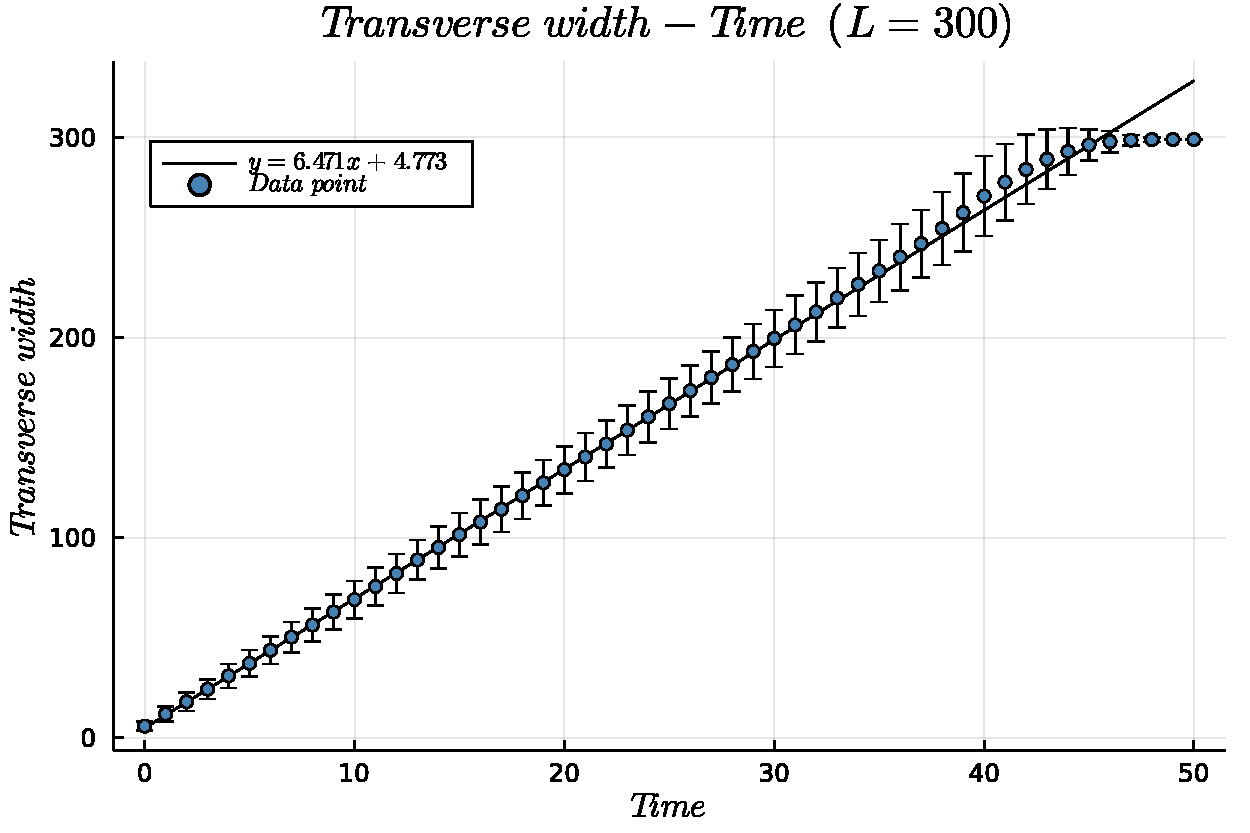
\includegraphics[scale = 0.4]{/Q3/Q3-L(t)}
        \label{fig:3.2}
        \caption{Competitive Ballistic Deposition for $L=300$.}
    \end{figure}

    As it is clear, the transverse width of the shrub grows linearly,
    until it becomes equal to the surface length.

    \section*{Problem 4}
    \textbf{Basic description:}

    Here we want to simulate the percolation of a binary defined network.
    In that case, we create a random binary network using the python networkx.
    Then we will check if there is a path between every node on the sides of the network.
    If we find a route, we will consider the percolation successful. And we check that for a range of P.
    So here is the result:

    \begin{figure}[!htb]
        \centering
        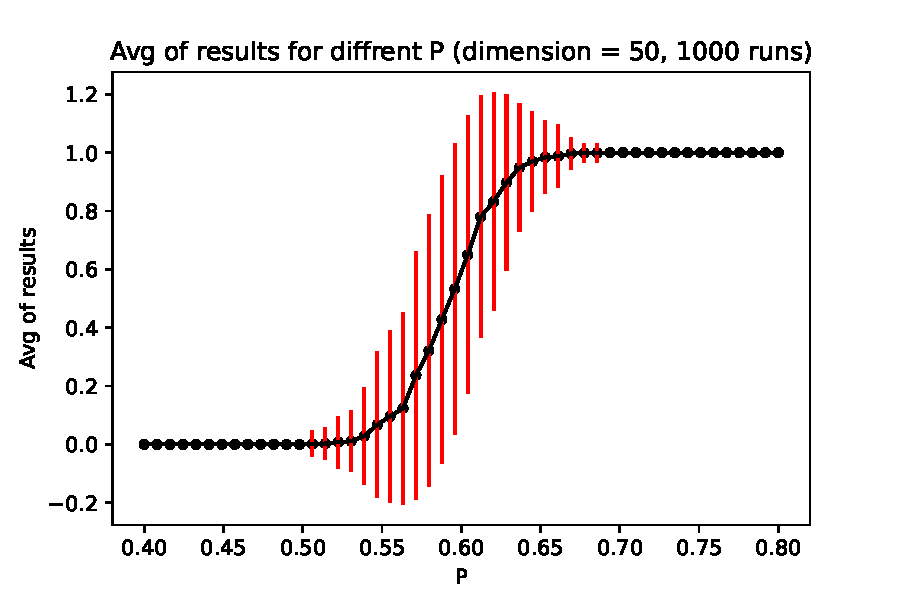
\includegraphics[scale = 0.5]{/Q4/Q4}
        \label{fig:4.1}
        \caption{The results of percolation for a range of P for 1000 runs.}
    \end{figure}

    \section*{Problem 5}
    \textbf{Basic description:}

    The coloring algorithm deployed as the question wanted.
    My program can find percolation in a binary network and return the result as 0 or 1.
    For some critical P (or at least near to critical point),
    I drew an animation of stages of the dynamic of percolation for colors.
    The results are available in the Q5 folder in the Figs folder.
\end{document}